
\section{Verlet Method}

This integration method was developed by Loup Verlet \citep{verlet} to solve the Newtonian equations in a many-body system. The procedure is simple and related to forward Euler integration. Using a Taylor expansion in (real!) time steps $\Delta t$ 

$$
\vec{x}\kl{t+\Delta t} = \vec{x}\kl{t} + \Delta t \vec{v}\kl{t} + \frac{1}{2}\Delta t^2 \dot{\vec{v}}+ ...
$$
$$
\vec{x}\kl{t-\Delta t} = \vec{x}\kl{t} - \Delta t \vec{v}\kl{t} + \frac{1}{2}\Delta t^2 \dot{\vec{v}}+ ...
$$
and adding the two expressions, one obtains
\begin{equation}
\vec{x}\kl{t+ \Delta t} = 2 \vec{x}\kl{t}- \vec{x}\kl{t-\Delta t} +\Delta t^2 \ddot{\vec{x}}\kl{t}.
\label{eq:verlet}
\end{equation}
Using Newton's equation, we can evaluate $\ddot{\vec{x}}\kl{t}$ as
$$
\ddot{\vec{x}}_i\kl{t} = \frac{1}{m_i} \sum_j{f_{i,j}\kl{t}}
\hspace{0.2cm} \text{with} \hspace{0.2cm} 
f_{i,j}\kl{t} = - \nabla V\kl{r_{i,j} \kl{t}},
$$
which we can insert in Eq. \eqref{eq:verlet}. Using $\Delta t \lesssim \frac{t_c}{10}$ (see Sec. \ref{subsec:contact_time}), we obtain the new position of the particle. 

Some general remarks about the Verlet method:
\begin{itemize}
\item Two time steps need to be stored ($t$ and $t-\Delta t$).
\item Velocities can be computed with $\frac{\vec{x\kl{t+\Delta t}} -\vec{x\kl{t-\Delta t}}}{2\Delta t}$.
\item The error of a single iteration is of order $\propto \Delta t^4$, i.e. it is globally a third order algorithm.
\item The numbers which are added are very different in magnitude ($\propto \Delta t^0$ and $\propto\Delta t^2$).
\item Improvable by systematical inclusion of higher orders (very inefficient).
\item The method is time reversible, which allows to estimate the error accumulation by reversing the process and comparing it to the initial conditions.
\end{itemize}



\section{Leap-frog Method}


In this case we will consider velocities at intermediate steps, and proceed similarly as in the forward Euler integration. 

$$
\vec{v}\kl{t+\frac{1}{2}\Delta t} =\vec{v}\kl{t-\frac{1}{2}\Delta t}  + \Delta t \cdot \ddot{\vec{x}}\kl{t}
$$
\begin{equation}
\vec{x}\kl{t+\Delta t} =\vec{x}\kl{t}  + \Delta t \cdot  \vec{v}\kl{t+\frac{1}{2}\Delta t}
\label{eq:leap}
\end{equation}
The leap-frog method has the same order of accuracy as the Verlet method, however both methods differ in the order in which the variables are integrated (see Fig \ref{fig:leap_verlet}).

The analogies and differences between the Leap-frog method

$$
\dot{\vec{v}}\kl{t+\Delta t} =\frac{f \kl{\vec{x}\kl{t}} }{m}
$$
$$
\vec{v}\kl{t+\Delta t} = \vec{v}\kl{t} + \Delta t  \cdot  \dot{\vec{v}}\kl{t+\Delta t}
$$
$$
\vec{x}\kl{t+\Delta t} = \vec{x}\kl{t} + \Delta t  \cdot \vec{v}\kl{t+\Delta t}
$$
and the more classical forward Euler integration
$$
\dot{\vec{v}}\kl{t+\Delta t} =\frac{f \kl{\vec{x}\kl{t}} }{m}
$$
$$
\vec{x}\kl{t+\Delta t} = \vec{x}\kl{t} + \Delta t  \cdot \vec{v}\kl{t}
$$
$$
\vec{v}\kl{t+\Delta t} = \vec{v}\kl{t} + \Delta t  \cdot \dot{\vec{v}}\kl{t+\Delta t}
$$
are clear: both rely on explicit forward integration. The update of the variables is then done in a different order. In the Leap-frog method the position is not updated using the previous velocity, as it is done in the usual Euler method.



\vspace{0.1cm}
\noindent
\begin{minipage}{\textwidth}
\begin{minipage}{.98\textwidth}
  \centering
  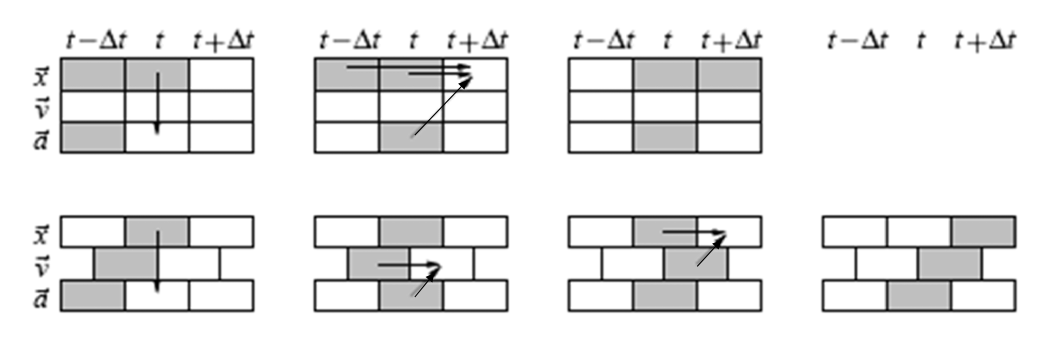
\includegraphics[width=0.95\textwidth]{pics/leap_verlet}
  \captionof{figure}{Comparison of Verlet (upper row) and Leap-frog (lower row) method.}
  \label{fig:leap_verlet}
\end{minipage}
\end{minipage}
\vspace{0.1cm}

Verlet and Leap-frog both use micro-canonical calculations in which energy is conserved. Therefore, for sufficiently small $\Delta t$, energy is usually conserved on average during a simulation. The fluctuations are due to round-off errors. Large fluctuations in energy are usually a hint for either the time step being too large or a bug in the code. The fluctuations of the energy can also be used to estimate the accuracy of the method. 

\vspace{0.1cm}
\noindent
\begin{minipage}{\textwidth}
\begin{minipage}{.98\textwidth}
  \centering
  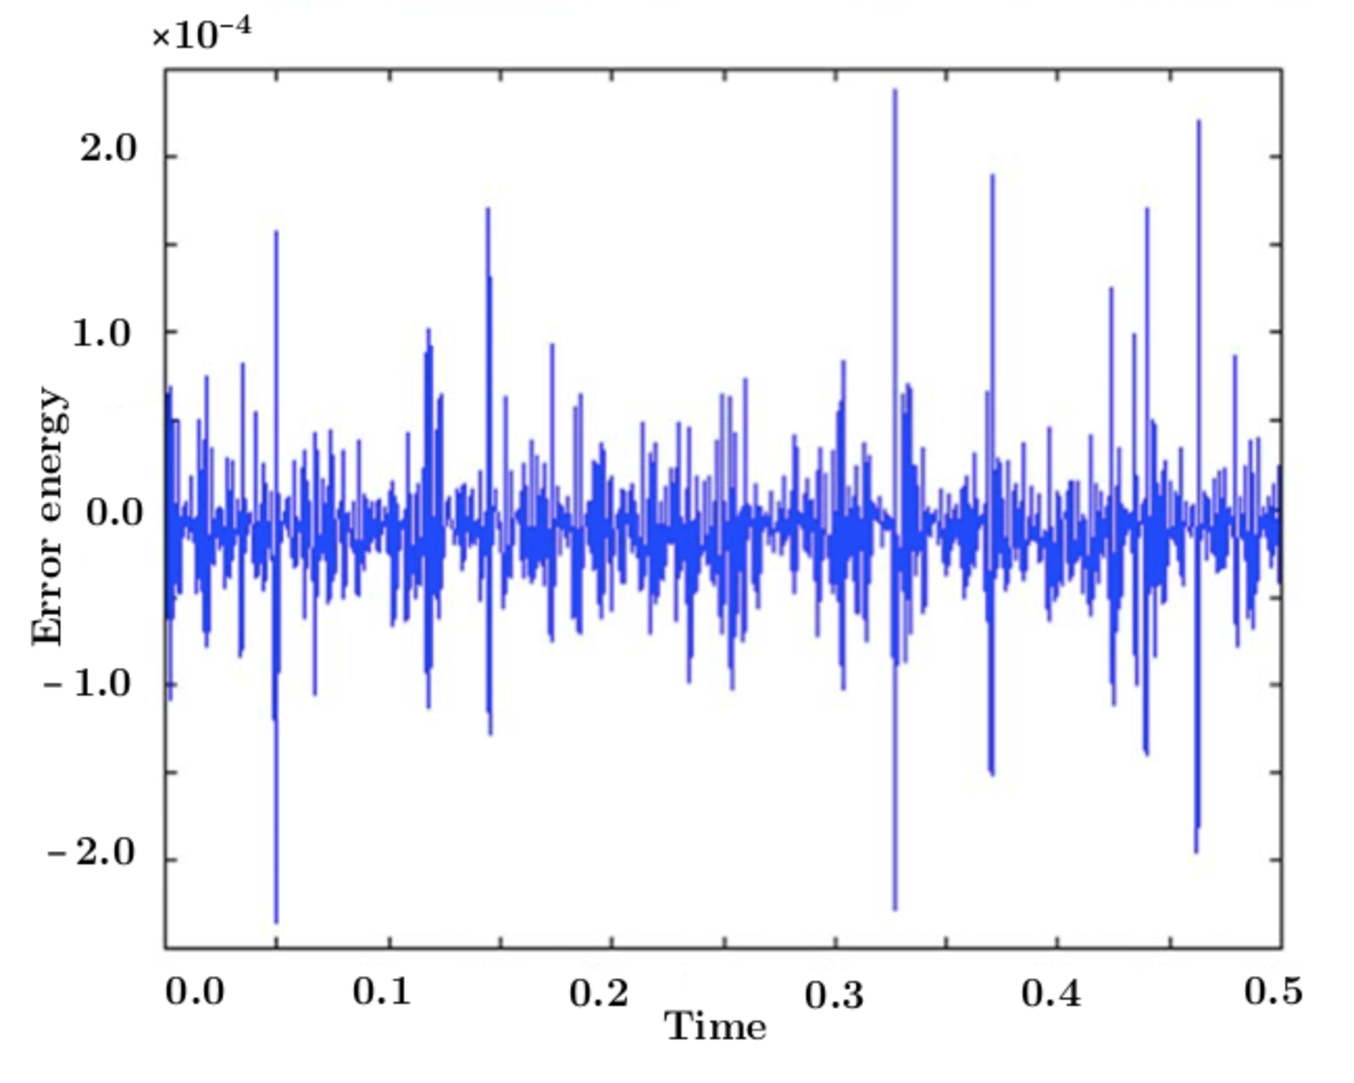
\includegraphics[height=250pt]{pics/energy_leap}
  \captionof{figure}{Energy in the Leap-frog method}
  \label{fig:energy_leap}
\end{minipage}
\end{minipage}
\vspace{0.1cm}

Since these methods are (mathematically speaking) completely time reversible, one can look at the change in the initial configuration after having simulated forward and then backward in time. The difference between the two configurations can be taken as a measure for the error of the method. 

Another approach consists in taking two initial configurations that  differ only slightly in the velocity or the position of a particle, and to observe the difference in time evolution of the two systems. Initially, both systems should behave similarly, but for larger simulation times, the systems will diverge (see Fig \ref{fig:divergence_leap}). The slope of $\log{\Delta E}$ (where $\Delta E$ is the energy difference between both systems) is an indicator of the precision of the method. The slope is called the \emph{Lyapunov exponent}, and it describes the divergence of the simulated trajectory from the true one. More generally, the Lyapunov exponents are related to chaos phenomena which we will not further discuss here. Symplectic integrators by contrast, have the remarkable property to estimate the true trajectory the better the larger the simulation time is. Moreover they preserve the total energy exactly \citep{yoshida}. This allows to simulate Hamiltonian systems such as the three-body problem very efficiently \citep{nagler}.

\begin{figure}[h!]
  \centering
  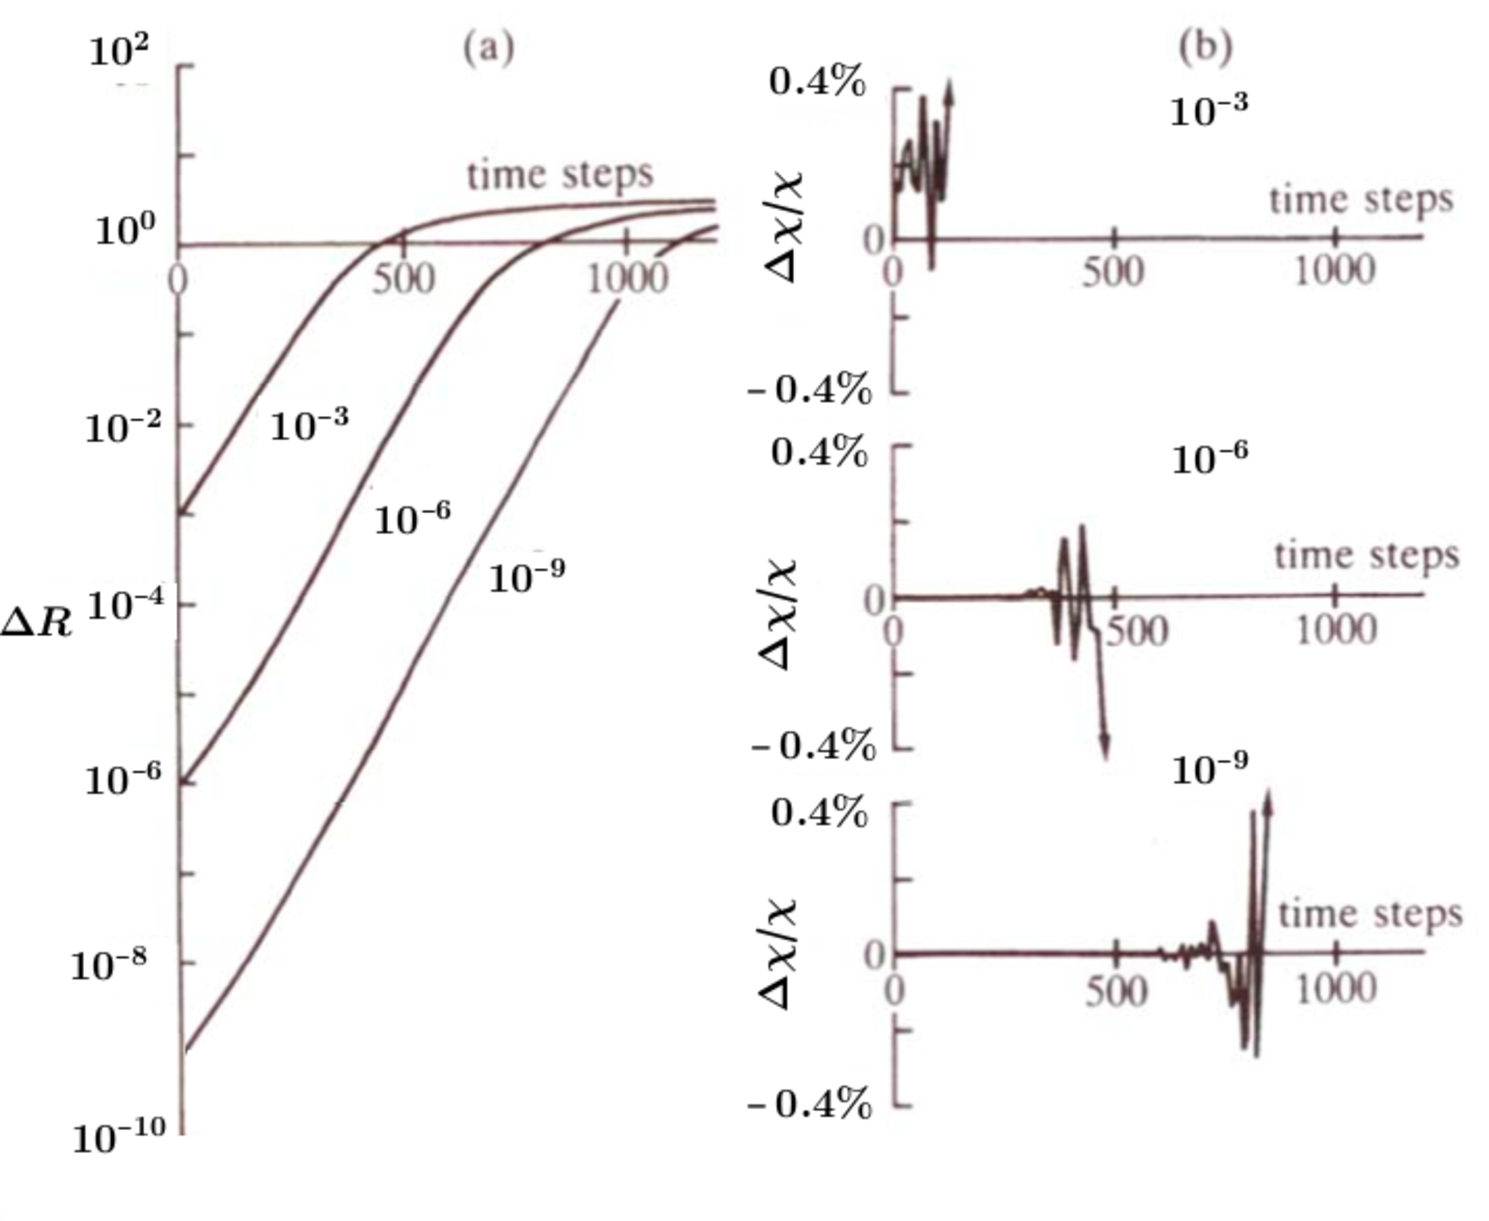
\includegraphics[width=0.6\textwidth]{pics/divergence_leap}
  \captionof{figure}{Comparison of the time development in systems with similar initial configurations. In each system one particle has been placed with an initial position shifted by $\Delta r$. The time evolution of the divergence of the trajectories has been depicted in the right panel, $a$. In the left panel, $b$, the time evolution of the relative energy difference in the the systems.}
  \label{fig:divergence_leap}
\end{figure}

\begin{figure}[h!]
  \centering
  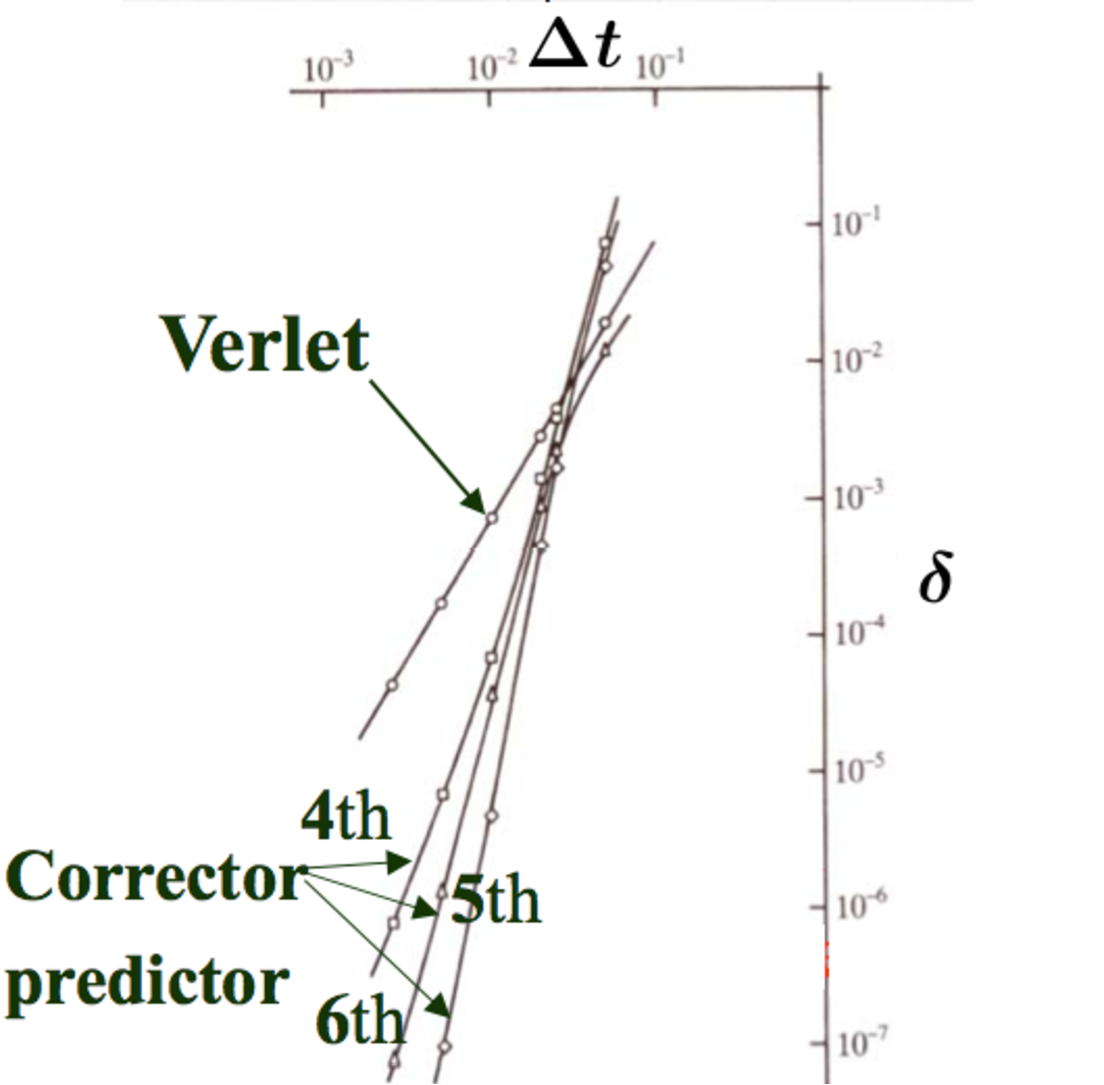
\includegraphics[width=0.5\textwidth]{pics/comp_verlet}
  \captionof{figure}{Comparison of the precision in the Verlet method and the predictor-corrector method of various order.}
  \label{fig:comp_verlet}
\end{figure}



\section{Optimization}

The systems used in MD simulations are usually composed of a large amount of particles. This represents a severe problem, as the computation of all possible pair interactions is very time consuming. e.g. the computation of the force from the potential. If the potential is a function of $\propto r^{y}$ and $y$ is an even number, one can omit the square root to compute the distance between the particles, as the exponent will cancel the square root.

If the potential is not a simple function and its calculation would imply a lot of tedious calculations, one can discretize the potential and sort the values in a look up table. The values can be recalled once the distance of the particle is calculated. The discretization should be chosen in such a way that no important feature is lost. For further precision one can linearly interpolate the bins and correct the values of the look-up table (Newton-Gregory interpolation).

In the case of short range potentials one could think of introducing a cut-off at a distance where the potential is negligible. Mind that this is a problem for $r^{-1}$ potentials since their contribution at very large distances is still not negligible. One can consider the idea of defining a new potential, shifted by a constant, such that it reaches exactly zero at the cut off. This won't affect the forces since any constant disappears when taking the gradient of the potential. Another idea is to interpolate the cut off with a linear (or quadratic) function that reaches zero in a finite distance. Mind that the function is continuous but not smooth at the connection. A careful programmer should be aware of this and address related troublesome situations with caution. Already the first derivative of the potential (i.e. the force) will present a discontinuity, and the second derivative even a divergence where the potential has been interpolated.
 
%BLABLA for MADIS, read till here!!

\subsection{Verlet Tables}

\vspace{0.1cm}
\noindent
%\begin{minipage}{\textwidth}
%\begin{minipage}{.55\textwidth}



%In order to reduce the amount of computations one can omit the computation of particle-particle interactions when they are negligible, therefore only particles that are in a certain range have to be considered. One approach to implement such a neighbourhood search is a \emph{Verlet table}, where only the particles in a certain range are stored. As the particles move with time, the table has to be updated regularly, with the updating time being dependent on the implementation of the Verlet table.

%%% By Madis %%%
% Verlet tables %

Brute force calculation of the particle-particle interactions between all $N$ particles is very costly, with complexity $O(N^2)$. For potentials decaying faster than $r^{-1}$ in distance it is reasonable to assume a cut-off range $r_C$ beyond which interactions are negligible.

%\end{minipage}\hfill
%\begin{minipage}{.4\textwidth}
\begin{wrapfigure}{r}{0.45\textwidth}
\vspace{-25pt}
  \centering
  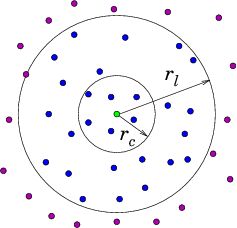
\includegraphics[width=0.4\textwidth]{pics/verlet_table}
  \captionof{figure}{Illustration of the Verlet table for the green particle. Blue particles are in the Verlet table, purple are not. \citep{MIT_numerical_methods}}
  \label{fig:verlet_table}
\end{wrapfigure}
%\end{minipage}
%\end{minipage}
%\vspace{-20pt}

\noindent Thus only interactions with particles in a certain neighbourhood have to be considered. The trick here is to find a efficient way of keeping track of which particles are in the neighbourhood. 

One approach is via using the so-called Verlet tables. For each particle we keep track of nearby particles inside a neighbourhood larger than the cut-off $r_l > r_c$ (see Fig \ref{fig:verlet_table}). Introducing such a buffer zone around the cut-off region allows us to update the neighbours list every $N_l$ time steps
\[
N_l= \frac{r_l - r_c }{\Delta t v_{max}},
\]  
where $V_{max}$ is the maximum velocity of a particle.

\clearpage % For the wrapfigure not to go over the page 

The Verlet table can be implemented using two one dimensional vectors LIST and POINT. In LIST sequentially stores all the neighbourhoods, and POINT[i] gives the index to the first particle in the neighbourhood of particle $i$. Thus the neighbourhood of particle $i$ is LIST[POINT[i]], ... , LIST[POINT[i+1]-1].   


%%% By Madis %%%
% Linked cell %

\subsection{Linked Cell Method}

%Another method is the \emph{linked cell method} \citep{art}.
The renewal of Verlet tables is still a $O(N^2)$ task, thus the above methods on the whole is still $O(N^2)$. For a truly $O(N)$ algorithm one can implement the \emph{linked cell method} \citep{art}. The simulation domain is discretised using a regular grid spacing $M$, that is larger than the double of cut-off range $r_c$


%\end{minipage}\hfill
%\begin{minipage}{.38\textwidth}
\begin{wrapfigure}{r}{0.45\textwidth}
  \vspace{-30pt}
  \centering
  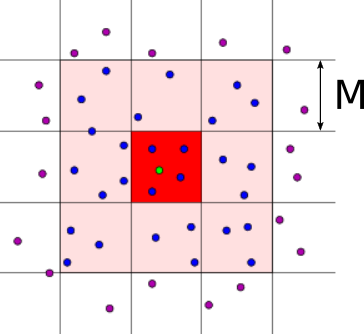
\includegraphics[width=0.4\textwidth]{pics/linked_cells_block}
  \captionof{figure}{The cells that contribute to the interaction are shaded. \citep{MIT_numerical_methods}}
  \label{fig:linked_cells}
  \vspace{-30pt}
\end{wrapfigure}
%\end{minipage}
%\end{minipage}
%\vspace{0.1cm}


\[
M > 2r_c.
\] 

%\vspace{0.1cm}
%
%\begin{minipage}{1.05\textwidth}
%\begin{minipage}{.6\textwidth}
\noindent We can now identify the cell in which each particle is located. Due to our choice of $M$, only the interaction to particles in a finite number of cells has to be computed, as particles in further cells will not interact with the respective particle. In d dimensions  there are $3^d$ cells of interest (See Fig \ref{fig:linked_cells}). On average we will have to test $N3^d \frac{N}{M^d}$ particles, many of which will not interact with the particle due to their distance. The advantage is that the update of cell populations can be done very efficiently. 


To look up which particle is in which cell during the computation, one stores in a vector \emph{FIRST} of length $\kl{\frac{L}{M}}^d$ ($L$ is the system size) for each cell $j$ the index of the (arbitrary) first particle in the cell. If the cell is empty, then \emph{FIRST}$\ekl{j}=0$. In a second vector \emph{LIST} of length $N$, the indices of the next particle in the same cell can be stored. If the particle $i$ is the last one in a cell, then \emph{LIST}$\ekl{i}=0$. See \ref{code:linked_cells} for an example on how to program a loop in C to go through all particles in a cell. When a particle changes the cell, \emph{FIRST} and \emph{LIST} can be updated locally, so that no loop over all particles is needed to update the configuration. The algorithm is thus of order $O\kl{N}$.

Additionally, this method is well suited for parallelization. One just has to us the grid to divide the system into domains, which are then each handled by a processor. Cells on the borders can be sent to the neighboring processors using MPI (see Fig. \ref{fig:linked_parallelization}).


\vspace{0.2cm}
\noindent
\begin{minipage}{\textwidth}
\begin{minipage}{\textwidth}
  \centering
  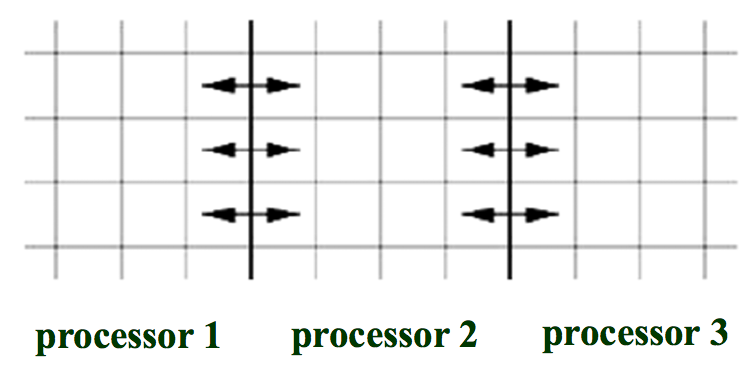
\includegraphics[width=.85\textwidth]{pics/linked_parallelization}
  \captionof{figure}{The System is divided into domains that are treated separately. Each domain is handled by a single processor unit and information can be exchanged using MPI.}
  \label{fig:linked_parallelization}
\end{minipage}
\end{minipage}
\vspace{0.1cm}









